%% OBJECT ORIENTED DESIGN

\section{Object-Oriented design}

\subsection{Design Overview}
The object oriented design was motivated by the class elicitation principle.
For example, there are classes for all of the key Petri net components, e.g.,
\texttt{Place}, \texttt{Transition}, \texttt{SourceArc}, \texttt{DestinationArc},
\texttt{Tokens}, and \texttt{PetriNetState} (an individual marking). Since a
Petri net is a mathematical construct, it is a natural fit for an ADT structure.

The project is divided into four packages as described in the following subsections.
The \texttt{logic.model} package handles all of the core logic for the Petri net
abstraction as described above. The \texttt{logic.utilities} package is responsible
for managing Petri net objects at run time, such as firing transitions and transferring tokens between places, i.e., representing markings, and generating
the coverability tree. The \texttt{io} package contains the classes responsible
for serializing Petri net objects to and from an XML representation. Finally, the
\texttt{ui} package encapsulates the user interface for visualizing Petri net 
objects, implemented using the Java Swing framework.

\subsection{Logic Modeling}
Text describing the Petri Net logic modeling class hierarchy presented in Figure~\ref{fig:logic-model-uml}.

\begin{figure}
	\centering
	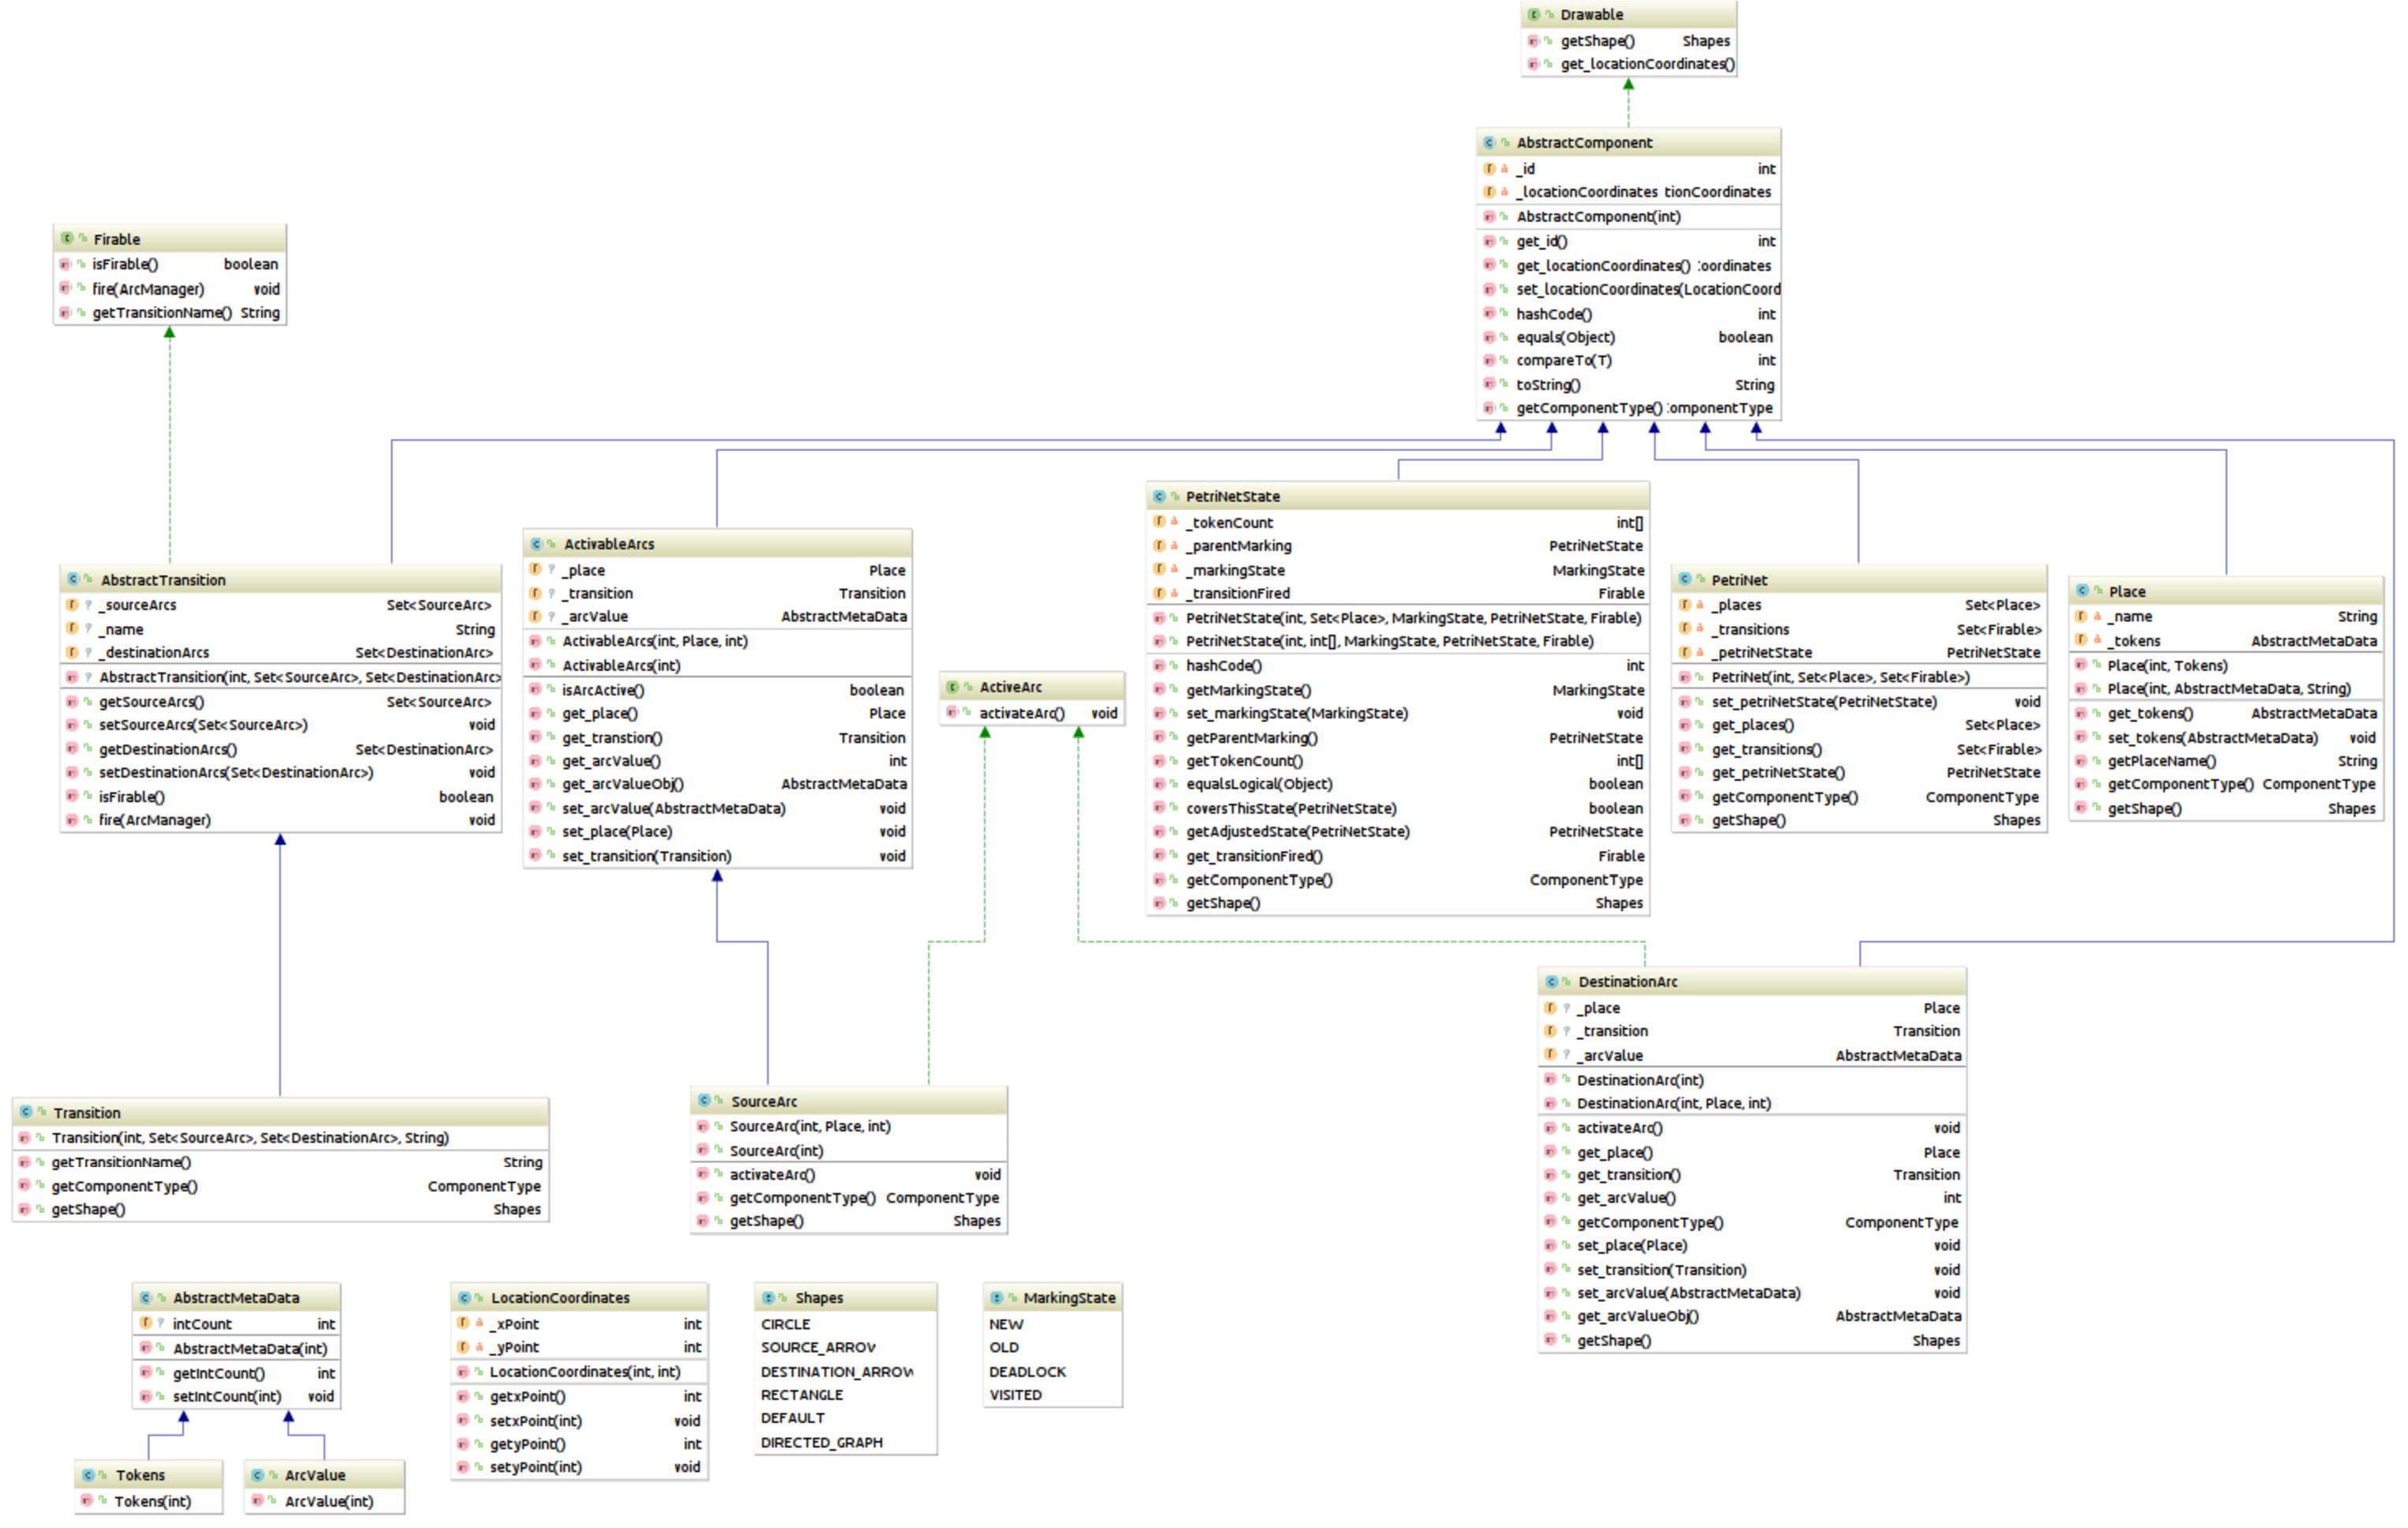
\includegraphics[width=1.0\columnwidth]{figures/logic-model-uml}
	\caption{UML class diagram for Petri Net logic modeling package.\label{fig:logic-model-uml}}
\end{figure}

\subsection{Logic Utilities}
Text describing the Petri Net logic utilities class hierarchy presented in Figure~\ref{fig:logic-util-uml}.

\begin{figure}
	\centering
	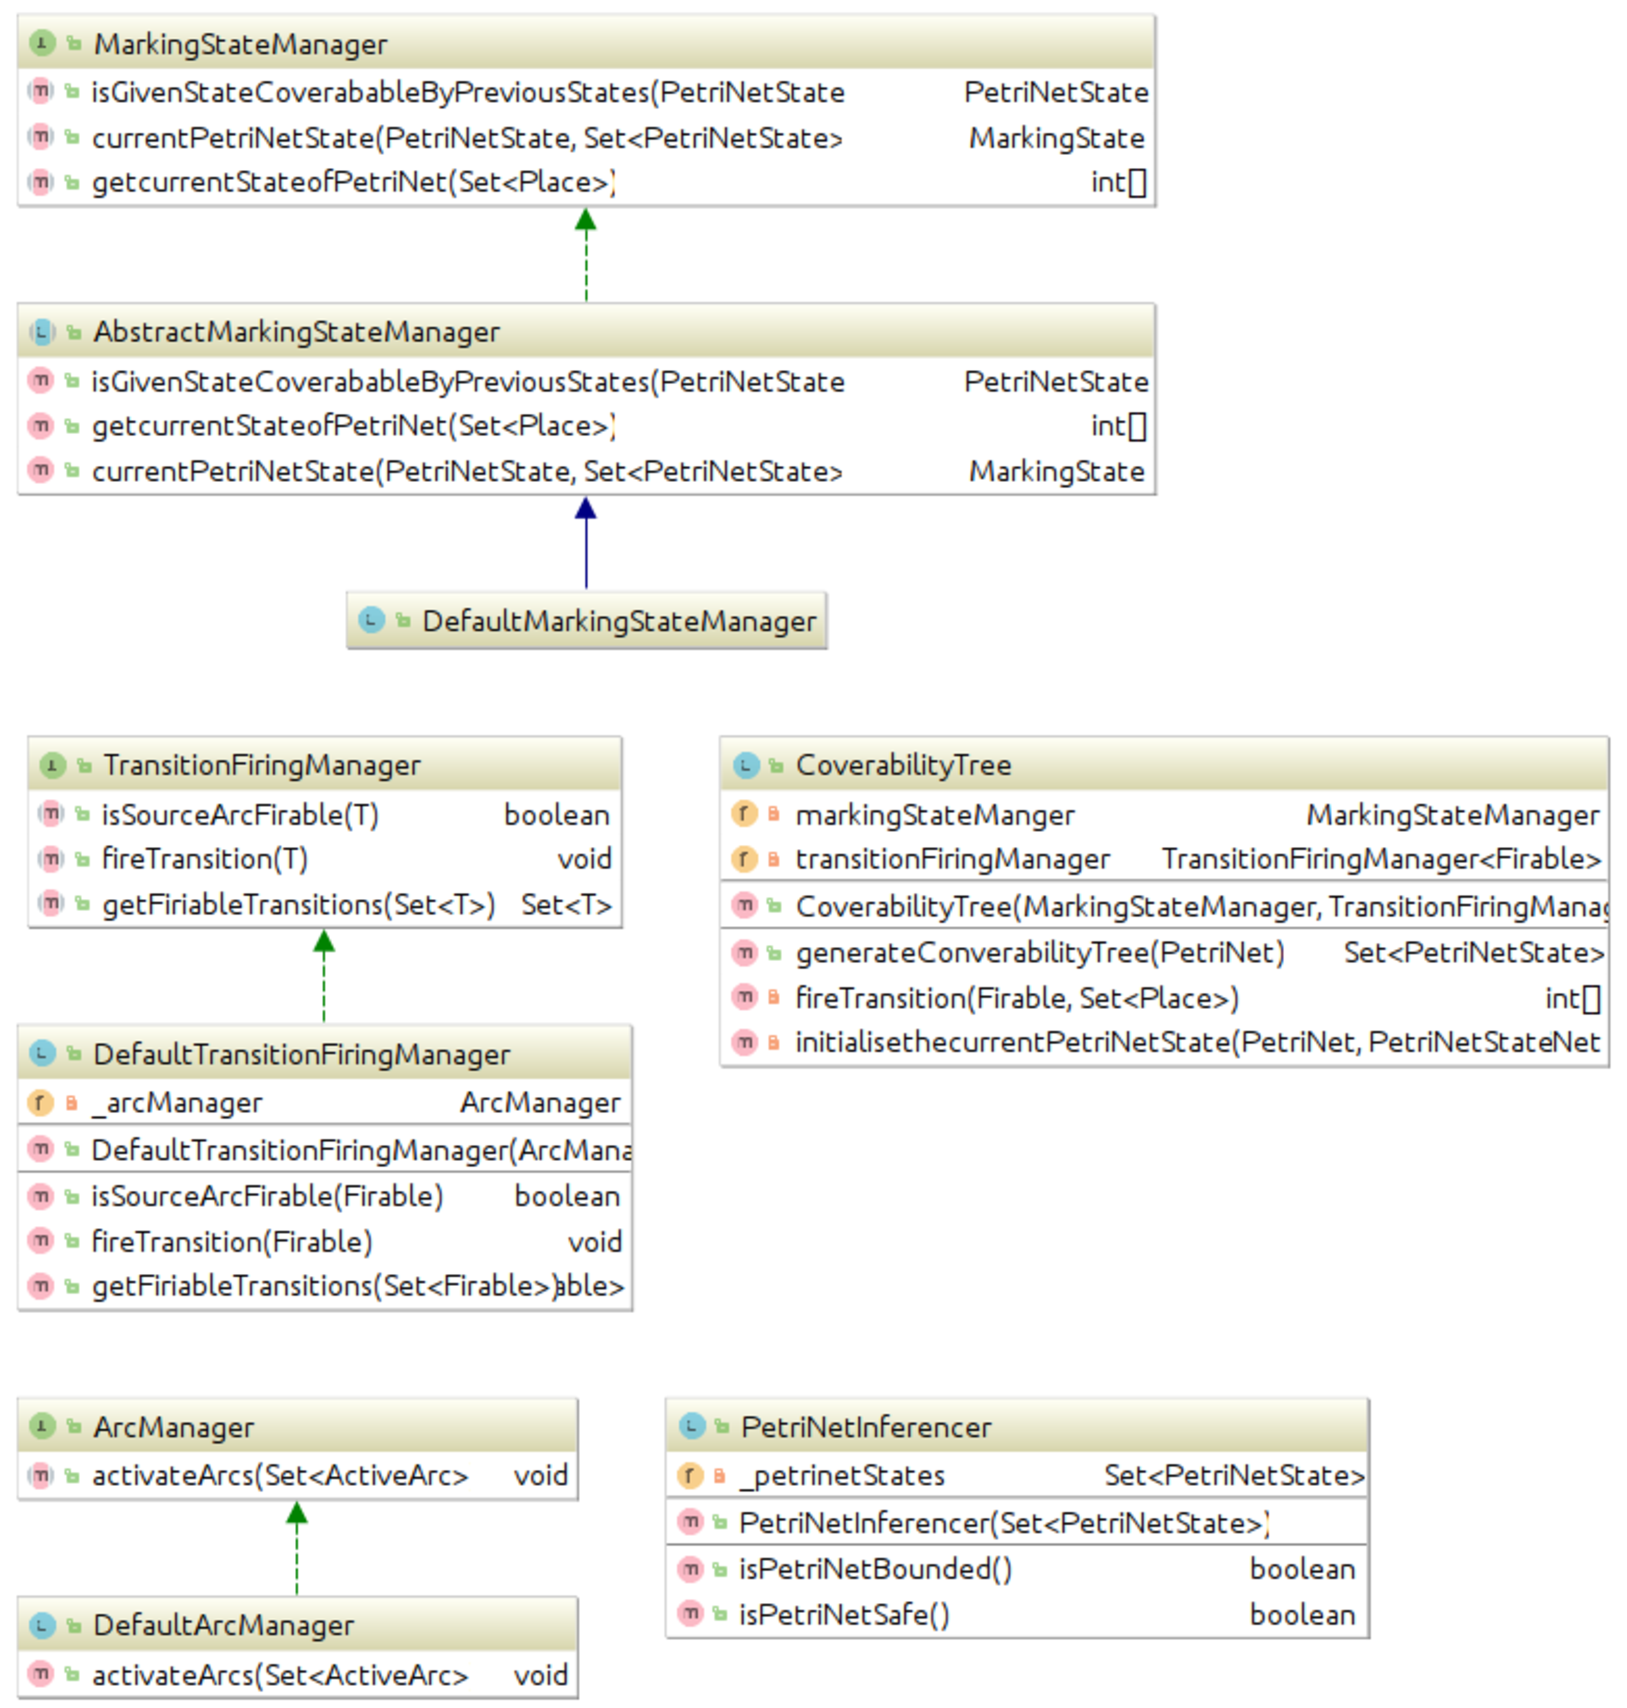
\includegraphics[width=1.0\columnwidth]{figures/logic-util-uml}
	\caption{UML class diagram for Petri Net logic utilities package.\label{fig:logic-util-uml}}
\end{figure}

\subsection{XML I/O}
The Petri net XML I/O class hierarchy is presented in Figure~\ref{fig:io-uml}.
The overall design is modeled after the \textit{Serialization Proxy} design
pattern. The purpose of this design pattern is to decouple the serialization
of an object from its implementation. For example, if the application must implement
the \textit{Serializable} interface without modifying the original source code.
In this case, the I/O package interacts with the classes in the \texttt{logic.model}
package, while treating it is a black box. In other words, it must serialize the
objects while only accessing their public methods.

The core of the I/O package is the abstract class \texttt{PetriSerializable},
responsible implementing the \texttt{Serializable} interface. It does not implement
the required \texttt{readObject} and \texttt{writeObject} methods directly, but
defers them to its concrete subclasses. Each of the subclasses is responsible
for serializing a particular Petri net component, and acts as an adapter to each
object via object composition, i.e., each serialization object obtains a reference
to the component it serializes.

The \texttt{PetriNetSerializer} class is the primary class in the hierarchy as it
is responsible for serializing or deserializing an entire Petri net object to
or from an XML stream. There is a corresponding concrete class for each
subcomponent, e.g., \texttt{PlaceSerializer}, \texttt{TransitionSerializer},
\texttt{SourceArcSerializer}, and \texttt{DestArcSerializer}.

There are also two utility classes that are essentially implementations of the
\textit{Factory Method} and \textit{Singleton} design patterns. The \texttt{IOComponentManager} singleton maintains the sets of components needed
for a Petri net object currently under construction while the \texttt{PetriNetSerializer.readObject}
method is running, and constructs new components as necessary. The
\texttt{XmlFactory} object performs the same role for XML components during
execution of the \texttt{PetriNetSerializer.writeObject} method.

The XML schema format implemented is a subset of PNML, the Petri Net Markup
Language. This enabled reuse of any Petri nets already defined in that format,
such as \textit{Producers and Consumers}, \textit{Dining Philosophers}, and
\textit{Communication Protocol}. Only the portions of the specification needed
for this class design were implemented. There are many XML parsers available for
Java, however the \textit{java.xml.parsers} package in the standard library
was selected for full compatibility and reliability.

When reading an XML stream, the \texttt{PetriNetSerializer} collects all place,
transition, and arc nodes into sets. It then processes places, arcs, and
transitions respectively to accommodate the \texttt{logic.model} implementation.
The parent-child relationships between components are mirrored in the XML document
by writing places, transitions, source arcs, and destinations. New nodes are
constructed by the \texttt{XmlFactory} as needed and appended to parent nodes.

\begin{figure}
	\centering
	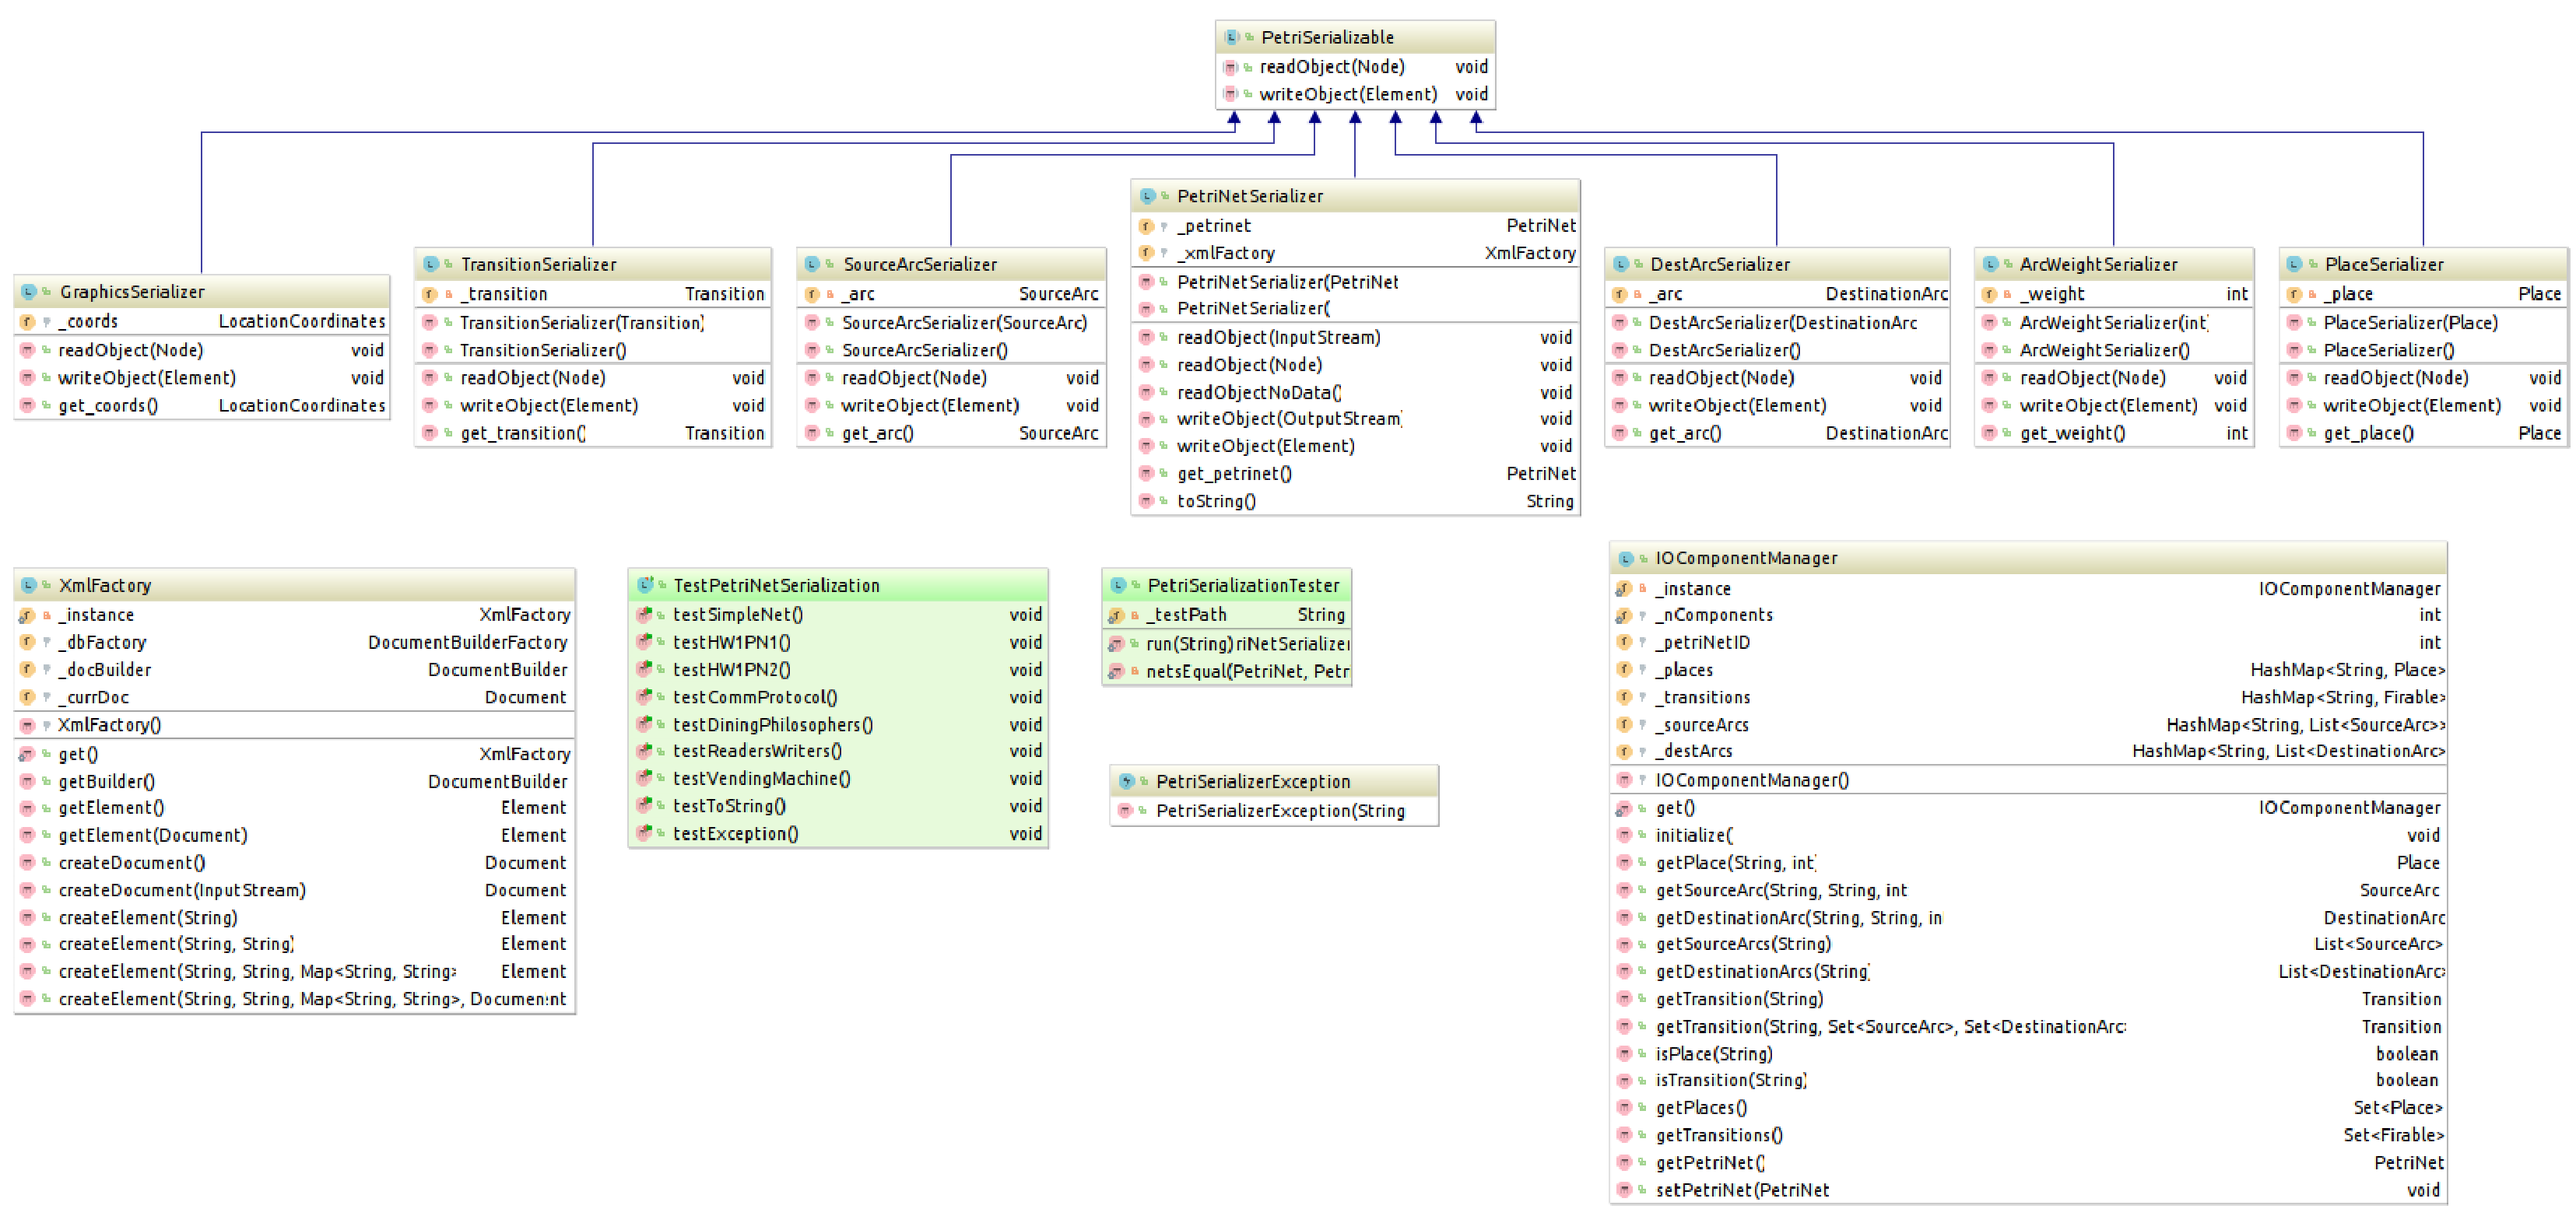
\includegraphics[width=1.0\columnwidth]{figures/io-uml}
	\caption{UML class diagram for Petri Net XML I/O package.\label{fig:io-uml}}
\end{figure}

\subsection{Graphical User Interface}
The Petri Net graphical user interface (GUI) class hierarchy is presented in Figure~\ref{fig:ui-uml}.

\begin{figure}
	\centering
	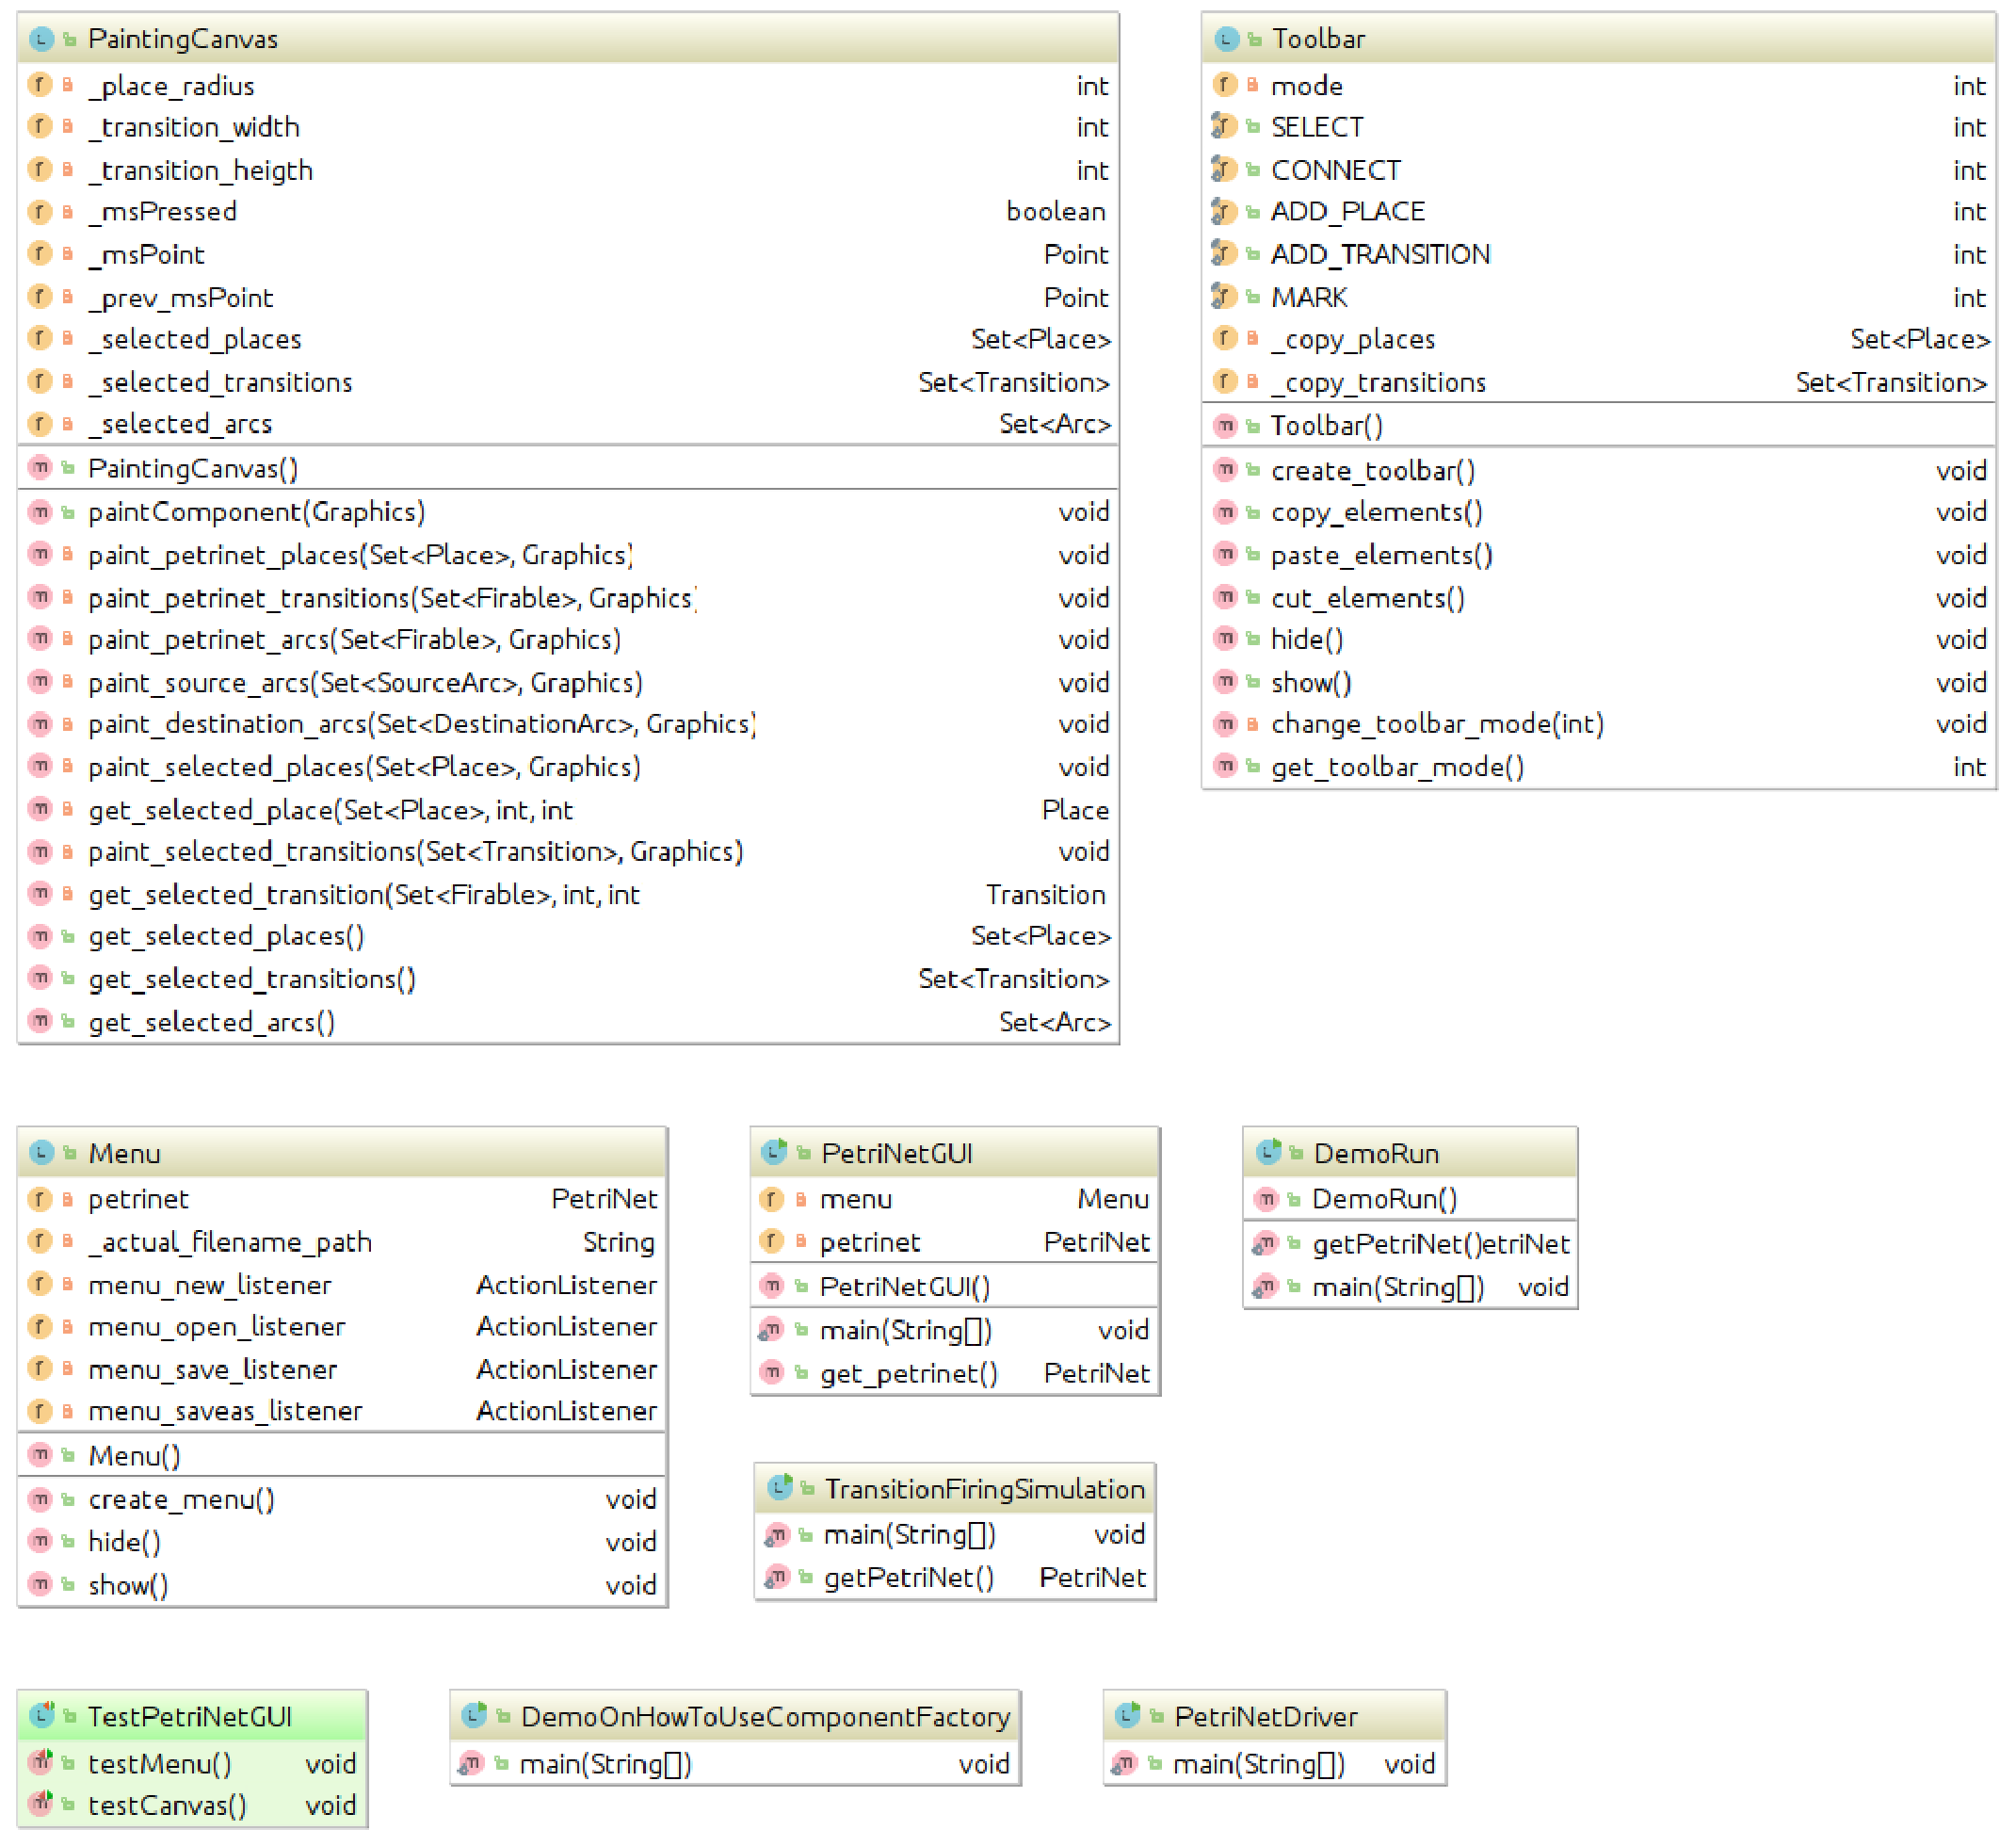
\includegraphics[width=1.0\columnwidth]{figures/ui-uml}
	\caption{UML class diagram for Petri Net graphical user interface (GUI) package.\label{fig:ui-uml}}
\end{figure}

As we know, neither Design By Contract nor Defensive programming is best suited for the class design. It solely depends on matter of time, the application context, class responsibility  and above all, the performance issue. So, we exploited both paradigms when we are distributing class responsibility, wherever they are feasible. The three key classes that we pick to justify our  conscience  on  how  the class  design follows the defined paradigm, will be explained below one by one.

\subsection{CoverabilityTree class}
{\bf{Class responsability: }} The main responsibility of this class is to implement the coverability tree drawing algorithm and return collection of all possible marking state along with their respective marking. 

{\bf{How the class follows the ADT: }} ADT is the specification of the class such that it defines the top level  structure of the class. The actual class is just the implementation of the ADT. According to ADT, class must have  functions with distinct behaviour and each function must be bounded by set of preconditions, that the client ensures, and the set of postconditions for which the function is obliged. The {\bf{CoverabilityTree}} has three that has distinct functionality and each of them has  set of precondition and postcondition.


\subsubsection*{\bf{public Set$<$PetriNetState$>$ generateCoverabilityTree(PetriNet petriNet)}}
\begin{itemize}[label={},leftmargin=2em]

\item {\bf{Method description: }} This method generates the coverability tree of the provided PetriNet. The coverability tree is represented as the collection of all possible PetriNetState.

\item {\bf{PreCondition: }} This method expects  the PetriNet instance, provided as a parameter, to be the valid PetriNet. The client must ensures that the PetriNet, he wants to pass to this method, is valid. The PetriNet class has a method named {\bf{validate()}}, which acts as a precondition check method.

\item {\bf{PostCondition: }} This method returns the coverability tree as a collection of PetriNetState, such that each entry in the collection will be a distinct PetriNetState which the petri net can be in, by firing a sequence of firable transition.  The returned  collected is formatted in such a way that client could create a graph structure from it. Each PetrinetState instance in the collection,  will hold  a reference to its parent while the first instance will point to null.

\end{itemize}

\subsubsection*{\bf{private int[] fireTransition(Firable firable, Set$<$Place$>$ places)}}
\begin{itemize}[label={},leftmargin=2em]

\item {\bf{Method description: }} This method fire the provided transition and returns the array of newly created token value.


\item {\bf{PreCondition: } } The method expects the firable instance  to be firable. The client must check either the instance   Firable Interface  is  firable or not by calling  {\bf{isFirable()}} method.


\item {\bf{PostCondition: }} The array return by the method has length equal to the number of places in the petri net and will contain current token count is each places after the provided transition is fired.

\end{itemize}


\subsubsection*{\bf{public PetriNet initialisethecurrentPetriNetState(PetriNet petriNet, PetiNetState petriNetState)}}

\begin{itemize}[label={},leftmargin=2em]
\item {\bf{Method description: }} This method initialize the provided PetriNet with the provided PetriNetState.


\item {\bf{PreCondition: }} The provided petriNetState must be valid. PetriNetState class provide a method {\bf{validate()}}, to test if the  PetriNetSate is valid or not. The client must call this method before calling  the above method  as a  precondition check.


\item {\bf{PostCondition: }} The method insures that the provided PetriNet is a valid PetriNet and initialize the token count in each places with the provided token value in petriNetState.

\end{itemize}



Seeing above we can say the the Coverability tree class is in accordance with the ADT specifications. Each method in this class is  design with design by contract approach. When means that, in the documentation, the postcondition and precondition is clearly specified in the documentation and method that provides precondition check is also expose publicly, so that the client could call it to validate the precondition. All three method of the class is in accordance with the command query separation principle. The first method  {\bf{generateConverabilityTree()}}  is  Query Method, because the method return the coverability tree of the petri net, without altering the state of the PetriNet. This method only process the the current state  of the petri net  to generate the coverability tree. The second method  {\bf{fireTransition}} is command method despite the fact that the method is returning the integer array. The method fires the provided transition, and update the token value of each affected places. In that sense, the method is updating the state of petriNet. Thus, this method is acting as a command method. The third method is also a command method, because it is also updating  the PetriNet state with the provided value of token for each places.  The result of this method is change in the state of PetriNet state and hence the method act as a Command method.


\subsection{PetriNetInferencer class}

\paragraph*{Class responsability: } The class hold the responsibility of performing various test on the petri net. It functionality to test  various properties of the PetriNet.

\paragraph*{How the class follows the ADT: } This class contains two method, and each of the method has distinct functionality and set of precondition and postcondition, which are explained below.




\subsubsection*{\bf{public boolean isPetriNetBounded() throws InvalidPetriNetStateException}}
\begin{itemize}[label={},leftmargin=2em]


\item {\bf{Method description: }}  The method test if the provided coverability tree is bounded or not. The coverability tree is represented as a collection of PetriNetState.



\item {\bf{PreCondition: }} The method expect  each PetriNetState  within the collection to be the valid PetriNetState. PetriNetState class expose a method validate() that act a precondition check method.



\item {\bf{PostCondition: }} The method returns false only if the coverability tree contains ‘w’ in any of the states token.

\end{itemize}


Seeing above, we can say that PetriNetInferner class is implemented in accordance with ADT specification. This class is design with defensive programming approach. The documentation do not expose the precondition, rather the method itself  take care of validating the precondition. The method only expose the postcondition. The first method, while iterating through the collection of PetriNet States, implicitly checks if the PetrinetState instance is valid or not and throws the exception if it is not valid. The second method is also doing the same. Defensive programming is computationally efficient for this class because, if we see the implementation of the two method, we will notice that, the implementation is  iterating over  each and every possible PetriNetState. So, it is far more efficient to make the single call to check, if the state is valid or not, than to make  client of this method, check the state validity for each PetriNetState instance manually as a precondition check.


We  have a super class by the name of AbstractComponentManager and   4  base class that extends this superclass. Each base class act as a concrete component manager for each element of PetriNet. For example, we have PlaceManager class that manages creation, edit, remove and search of the place, also we have TransitionManager that manages creation, edit, remove and search of the transition and so on. We formally define AbstractComponentManager as a class designated for handling various operations related to  elements of Petrinet. AbstractComponentManager is a generic class, it provides, on the house, various common functionality  that is reusable by concrete component manager classes. Functionality like findByComponentId, getLastComponentId, clear are  reused by all the base classes. It also expose some abstract methods like getComponent, copyComponent, attachComponentToItsParent, updateComponentMetaData, getComponents. The implementation of these abstract method is dependent upon the element type the base class is supposed to work with. For example, the base class that works with Places, will implement these method, in accordance to Place element, and by the base class that works with DestinationArc element.

Each subclass in the defined inheritance structure implies both model-view as well as type-view structure.  First the each base class can reuse  the method provided by the base class and if it wants to modify the behaviour of any existing method, it can do so by overriding it. The inheritance structure follows the open close  principle and all the base class is being facilitated because of this.
In order to explain  the implication of  type-view model, consider the {\bf{ComponentFactory}} class.  Component factory class is design based on factory design pattern. This class contain basic method that allows basic operation to be done on the petri net element in  generic way. Let’s consider the simple method called {\bf{getComponent()}}.  If we see the implementation of getComponent() method, we can see, how it has exploited the concept of dynamic binding in it.  The type of component return by this method is independent of the component manager type it  dealing with at compile time. Java runtime call the right getComponent method on right base class of AbstractComponentManager  at the execution time, and return the appropriate  component, the client is expecting. This dynamism is achieved because of remarkable feature of object oriented language called {\bf{Polymorphism}}.  Thus, we can visualize  the implication of both model-view and type-view concept being used, because of above inheritance behaviour. 













